\documentclass{beamer}

\mode<presentation>
{
%\usetheme{Warsaw} %ok
%\usetheme{Rochester}
%\usetheme{Madrid}
%\usetheme{Pittsburgh}
%\usetheme{Antibes}
%\usetheme{Montpellier}
%\usetheme{Berkeley}
%\usetheme{PaloAlto}
%\usetheme{Goettingen}
%\usetheme{Marburg}
%\usetheme{Hannover}
%\usetheme{Berlin}
%\usetheme{Ilmenau}
%\usetheme{Dresden}
%\usetheme{Darmstadt}
\usetheme{Frankfurt} %ok
%\usetheme{Singapore} %ok
%\usetheme{Szeged}
%\usetheme{Copenhagen} %ok
%\usetheme{Malmoe}
\setbeamercovered{transparent}
}
% Choose color scheme
%
%\usecolortheme{default}
%\usecolortheme{sidebartab}
%\usecolortheme{albatross}
%\usecolortheme{beetle} 
%\usecolortheme{crane}
%\usecolortheme{dove} 
%\usecolortheme{fly} 
%\usecolortheme{seagull}
%\usecolortheme{lily}
\usecolortheme{orchid}
%
\usepackage{graphicx}
\usepackage[english]{babel}
\usepackage[utf8]{inputenc}
\usepackage{color}

\def\etal{\emph{et al}.}
\def\v#1{\protect\vec #1}
\definecolor{mygreen}{rgb}{0.0,0.6,0.1}
\newcommand{\ok}[1]{{\small \scriptsize  \color{mygreen} #1}} 
\newcommand{\bad}[1]{{\small \scriptsize  \color{red} #1}} 

%==============================================================================

\title{Recognizing human actions in still images:
a study of bag-of-features and part-based
representations}
\author{Vincent Delaitre, Ivan Laptev and Josef Sivic}

\begin{document}

\maketitle

%==============================================================================
\begin{frame}
\tableofcontents
\end{frame}

%==============================================================================
\section{Introducing a new dataset}
\begin{frame}
\frametitle{Introducing a new dataset}
We collected a new challenging dataset for real-life human actions. 

It is composed of 968 images collected from Flickr representing natural variations in terms of 
camera view-point, human pose, clothing, occlusions and scene background.

Pictures are distributed among 7 different classes: 
\begin{itemize}
\item Interacting with a computer
\item Taking a photograph
\item Playing music
\item Riding bike
\item Riding horse
\item Running
\item Walking
\end{itemize}

\end{frame}

%------------------------------------------------------------------------------

\begin{frame}
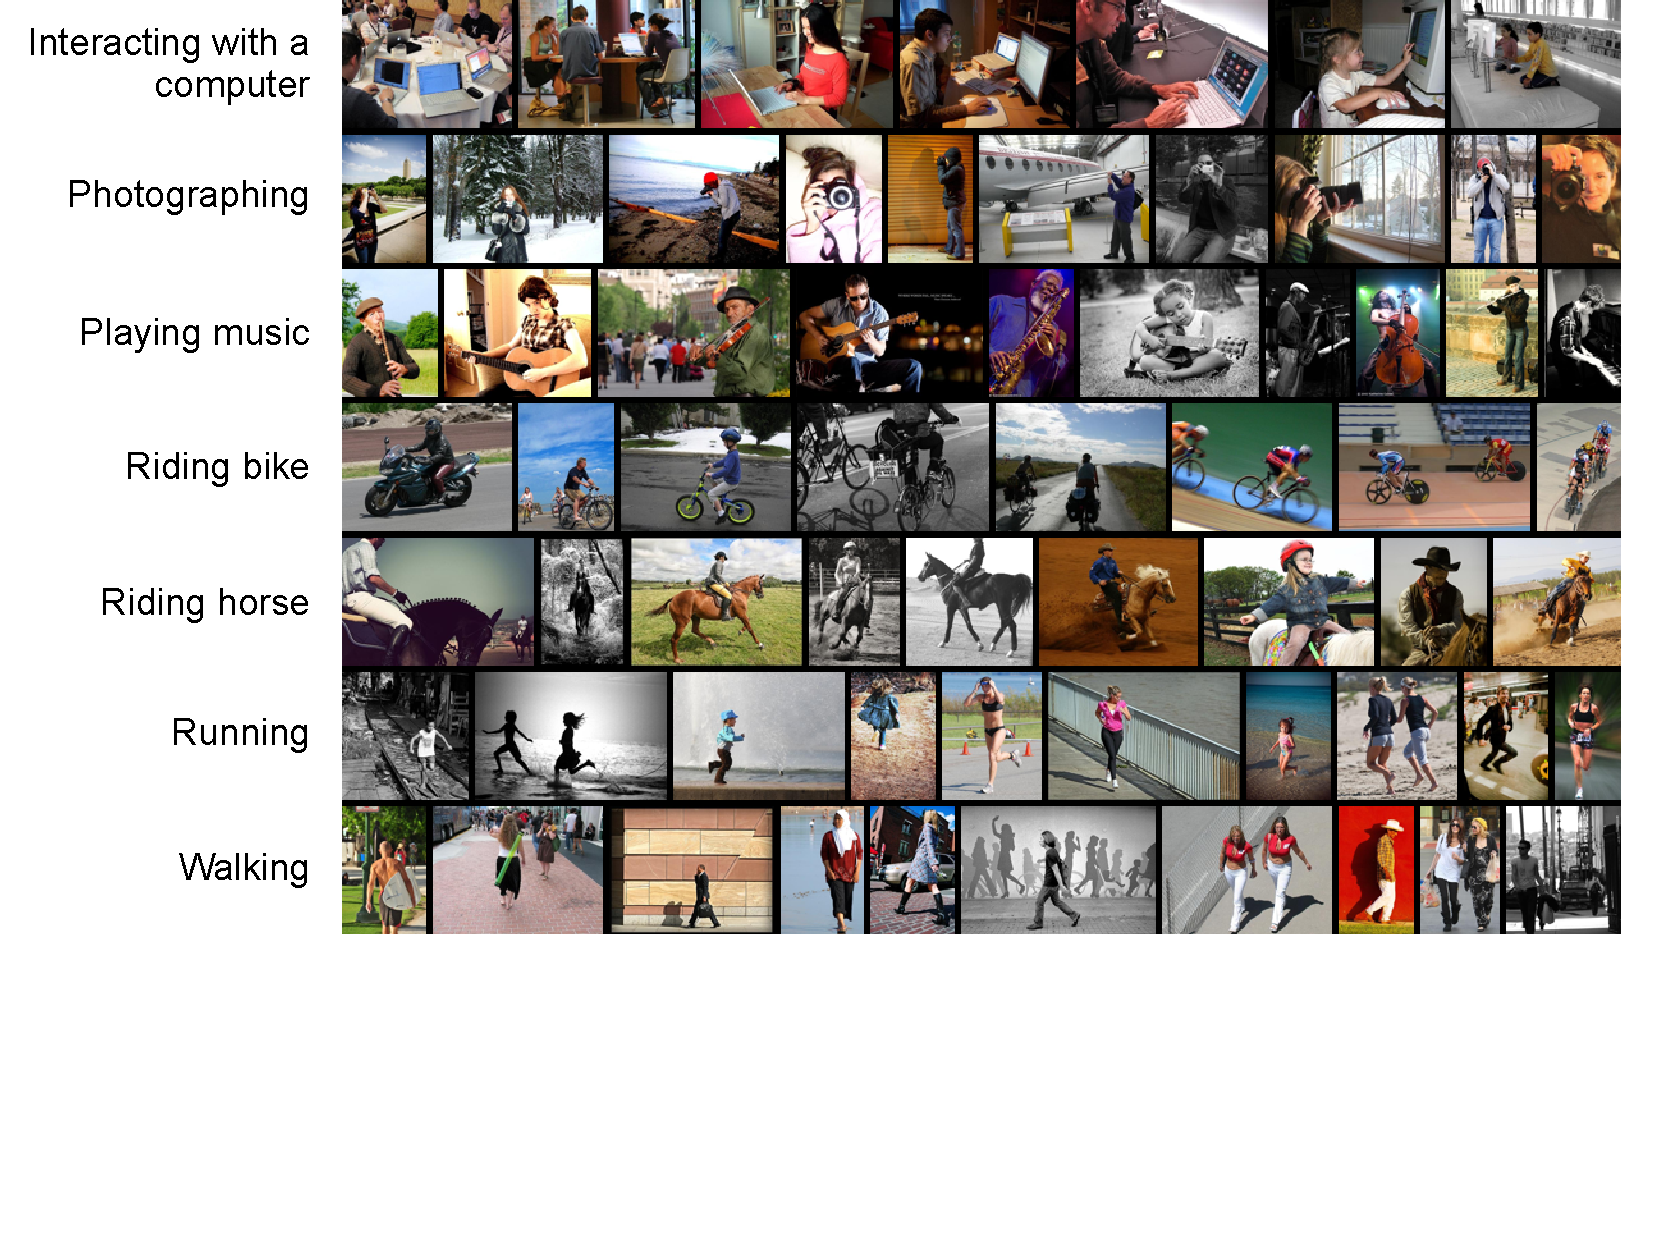
\includegraphics[width=1\linewidth]{figs/my_dataset_cropped.pdf}
\end{frame}

%------------------------------------------------------------------------------

\begin{frame}
\frametitle{Classification task}
Each person is annoted with a bounding box (smallest rectangle containing its visible pixels)
and the action being executed.

\vspace{0.3cm}
In the following, we are interessted in the 7-class classification problem.
The training set consists in 70 images of each type of action, so that at least 48 images
per class remain for test.

\vspace{0.3cm}
We mesure the performances using:
\begin{enumerate}[i]
\item {\em the classification accuracy}: average of the diagonal of the confusion table
\item {\em the mean average precision (mAP)}: mean area under the precision-recall curve of each 1-vs-all classifiers.
\end{enumerate}

\end{frame}

%------------------------------------------------------------------------------

%==============================================================================
\section{Bag-of-features classifier}
\begin{frame}
\tableofcontents[currentsection]
\end{frame}


\begin{frame}
\frametitle{Bag-of-features classifier}
Here we investigate the influence of various type of parameters in the classifier
performances:

\begin{itemize}
\item \textbf{Image representation}: Images are represented using the spatial pyramid 
representation from Lazebnik~\etal~.
\item \textbf{SVM Classification}: We use 1-vs-all classification scheme. We investigate
the efficiency of different kernels.
\item \textbf{Using context information}: We analyse the impact of the context using
information provided by the bounding box.
\end{itemize}

\end{frame}

%------------------------------------------------------------------------------
\subsection{Image representation}

\begin{frame}
\frametitle{Bag-of-features classifier: Image representation}

\begin{itemize}
\item Features are extracted from multi-scale dense sampled SIFT descriptors.
\item Visual vocabulary is built from k-means clustering. Size of the dictionnary $K \in \{256, 512, 1024, 2048, 4096\}$.
\item Following Lazebnik~\etal~, we use a 2 levels spatial pyramid: image is divided into $1 \times 1$, $2 \times 2$ and $4 \times 4$
grids of cells leading to a $(1+4+16)K = 21K$ dimensional reprensation of an image.

\end{itemize}

\center
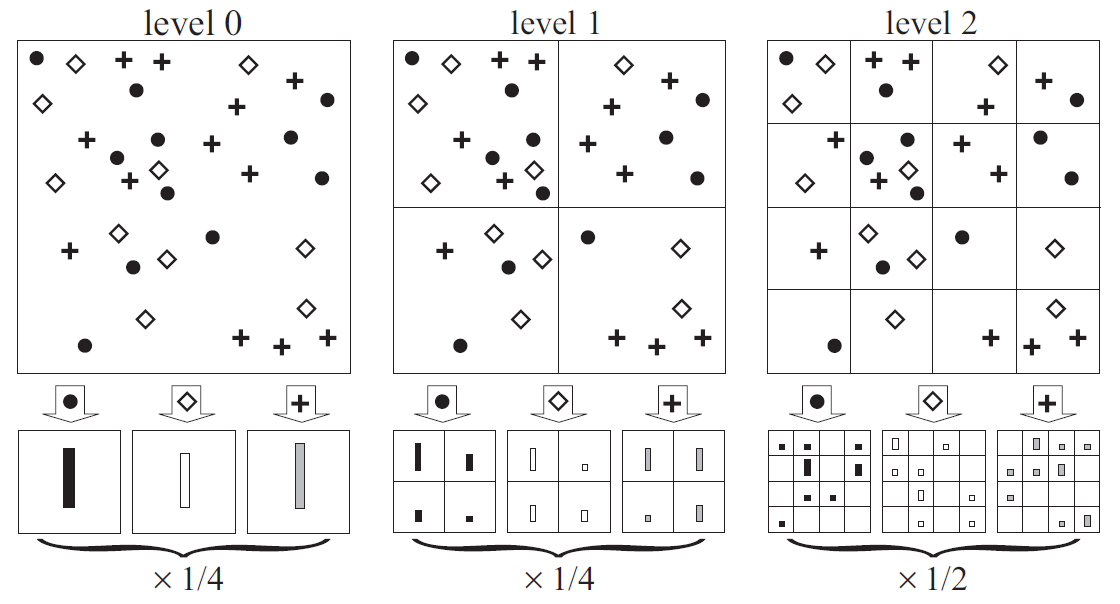
\includegraphics[width=0.5\linewidth]{figs/spatial_pyramid.png}

\end{frame}

%------------------------------------------------------------------------------

\subsection{SVM Classification}
\begin{frame}
\frametitle{Bag-of-features classifier: SVM Classification}

Classification is performed with
the SVM classifier using the 1-vs-all scheme, which, in our experiments, resulted in a small but consistent improvement
over the 1-vs-1 scheme. 
 
We investigate four different kernels: 
\begin{enumerate}
\item the histogram intersection kernel, given by $\sum_i \min(x_i,y_i)$;
\item the $\chi^2$ kernel, given by $\exp\{\frac{1}{\gamma} \sum_i \frac{(x_i-y_i)^2}{x_i+y_i}\}$; 
\item  the Radial basis function (RBF) kernel, given by  $\exp\{\frac{1}{\beta} \sum_i (x_i-y_i)^2\}$; and
\item the linear kernel given by $\sum_i x_i y_i$,
\end{enumerate}

where $\v x$ and $\v y$ denote visual word histograms of images $X$ and $Y$, and $\gamma$ and $\beta$ are
kernel parameters.

\end{frame}


%------------------------------------------------------------------------------ 

\subsection{Using context information}
\begin{frame}
\frametitle{Bag-of-features classifier: Using context information}

We consider the following four approaches:
\begin{enumerate}
\item[A.] {\bf \color<2,3,4>{gray}``Person"} 
\only<1>{Images cropped to $1.5 \times$ the size of the bounding box. Resize so that the larger dimension is 300 pixels.}

\item[B.] {\bf \color<1,3,4>{gray} ``Image"} 
\only<2> {Histograms are computed on the full image. Image resized so that the larger dimension is 500 pixels.}

\item[C1.] {\bf \color<1,2,4>{gray} ``Person+Background''} 
\only<3> {Background is represented only with a BOF histogram. Kernel values between two images $\v x$ and $\v y$ 
is the sum of two kernels over the foreground and the background: $K(\v x,\v y)=K(\v x_f,\v y_f)+K(\v x_b,\v y_b)$}

\item[C2.] {\bf \color<1,2,3>{gray} ``Person+Image''}
\only<4> {This setup is similar to C1, however, instead of the background
region, 2-level spatial pyramid representation of the entire image is used.}

\end{enumerate}

\only<1-2>{
$~$

$~$
}

\only<4>{
$~$
}

\only<1> {\hspace{1cm}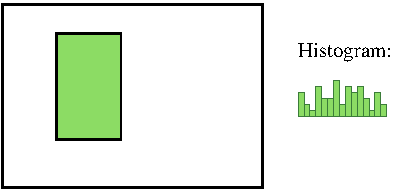
\includegraphics[scale=0.9]{figs/histo_person.pdf}}
\only<2> {\hspace{1cm}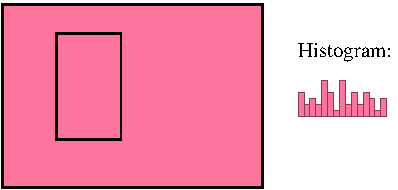
\includegraphics[scale=0.9]{figs/histo_image.pdf}}
\only<3> {\hspace{1cm}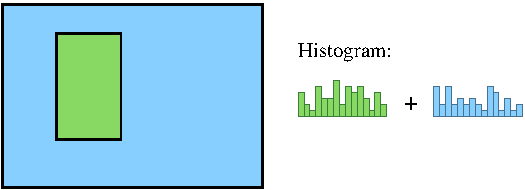
\includegraphics[scale=0.9]{figs/histo_person_backgnd.pdf}}
\only<4> {\hspace{1cm}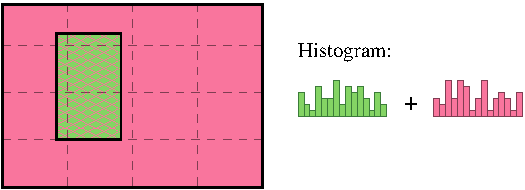
\includegraphics[scale=0.9]{figs/histo_person_image.pdf}}

\end{frame}

%------------------------------------------------------------------------------ 

\subsection{Results}
\begin{frame}
\frametitle{Bag-of-features classifier: Results}

\begin{figure}[tbp]
\centering \small
\begin{tabular}{cc}
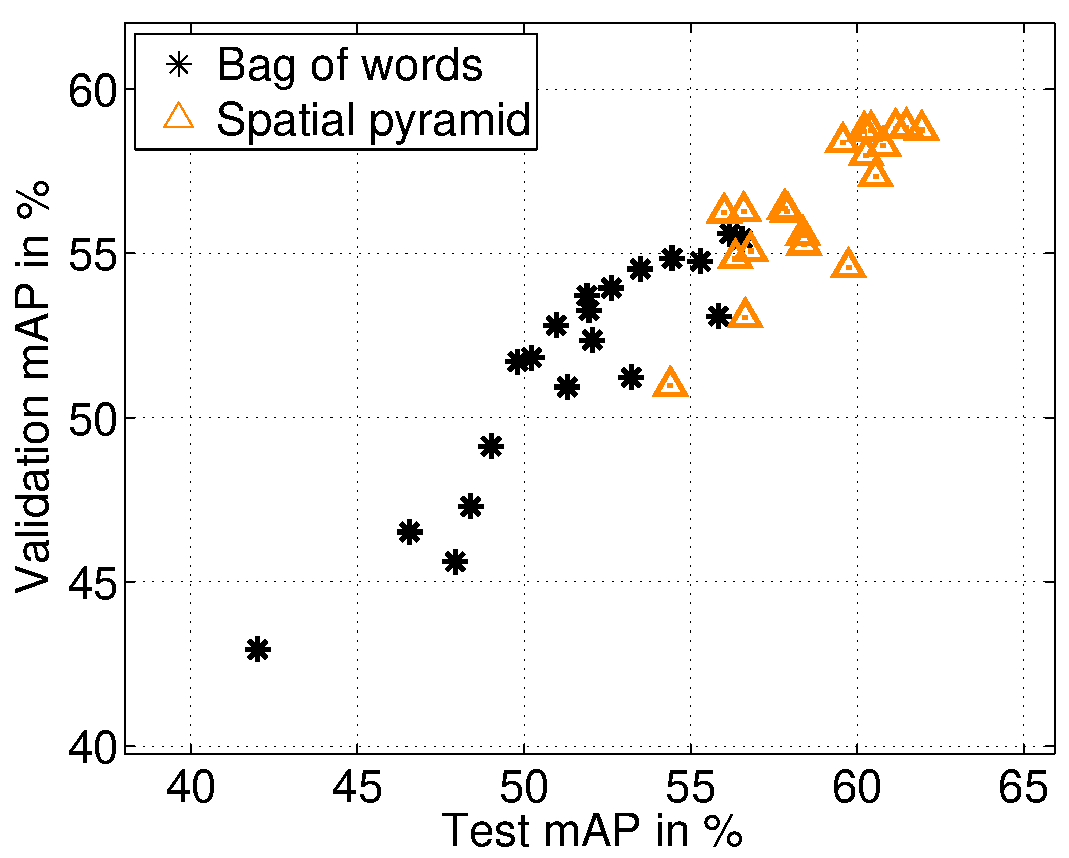
\includegraphics[height=.3\linewidth]{figs/caseA_error_BOF_PYR.pdf} &
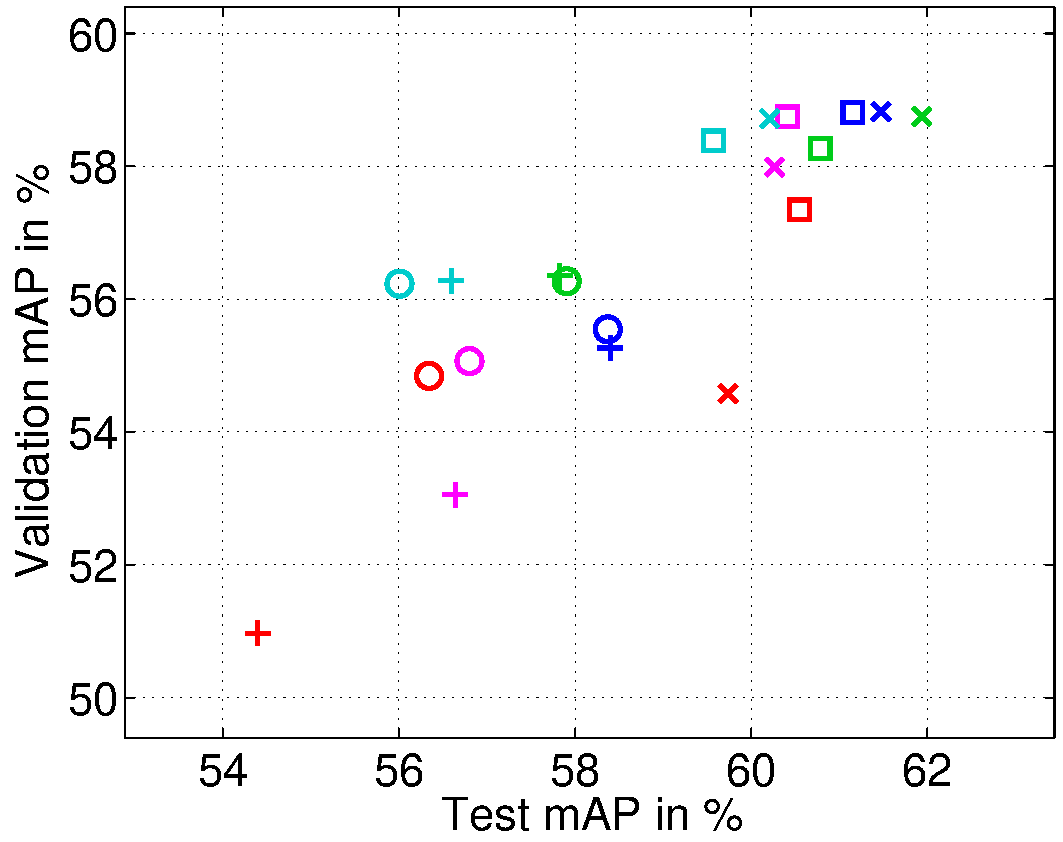
\includegraphics[height=.3\linewidth]{figs/caseA_error_PYR.pdf}
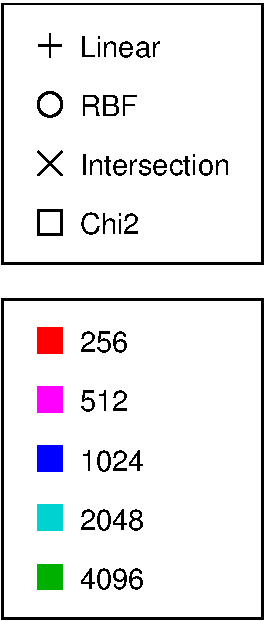
\includegraphics[height=.3\linewidth]{figs/legend.pdf}\\
(a) & (b)  \\
\end{tabular}
\caption{Classification performance (cross-validation mAP vs. test mAP) for different parameter settings for the method ``A. Person". (a) 2-levels spatial pyramid vs. the bag-of-feature representation.  (b) Classification performance for different combinations of kernels  and vocabulary sizes using the 2-levels spatial pyramid representation. The standard deviation of the validation mAP is typically 2-3\%.
}
 \label{fig:caseA}
\end{figure}

\end{frame}

%------------------------------------------------------------------------------ 

\begin{frame}
\frametitle{Bag-of-features classifier: Results}

In the following we use the best parameters for validation time of method ``A. Person": visual dictionnary size K = 1024 and intersection kernel.
We analyse the influence of context:

\begin{table}[tbp]
\centering
%\rowcolors[]{1}{white}{gray!10}
\begin{tabular}{|l|c|c|}
\hline
 Method                   &$~~~$mAP$~~~$&  Accuracy  \\ \hline 
 A.  Person          &  $61.48$ &  $59.08$ \\ \hline 
 B.  Image           &  $62.83$ &  $60.24 $ \\ \hline 
 C1. Person+Background&  $63.96$ &  $62.65$ \\ \hline 
 C2. BOF Person+Image     &  $70.43$ &  $67.01$ \\ \hline 
\end{tabular}
\caption{The overall classification performance for the different methods.}
\label{tab:methods}
\end{table}


\end{frame}

%==============================================================================
\section{Discriminatively trained part-based model}
\begin{frame}
\tableofcontents[currentsection]
\end{frame}

%------------------------------------------------------------------------------ 
\subsection{The latent SVM}
\begin{frame}
\frametitle{The latent SVM}

\end{frame}

%------------------------------------------------------------------------------ 
\subsection{Combining part-based model and bag-of-features}
\begin{frame}
\frametitle{Combining part-based model and bag-of-features}

\end{frame}

%------------------------------------------------------------------------------ 
\subsection{Results}
\begin{frame}
\frametitle{Results}

\begin{table}[tbp]
\centering
%\rowcolors[]{1}{white}{gray!10}
\begin{tabular}{|l||c|c|c|}
\hline
 Action /  Method & $~~$BOF C2$~~$ & $~~$LSVM$~~$ & $~$LSVM+ BOF C2$~$ \\ \hline 
(1) Inter. w/ Comp. & ${\bf 84.21}$ & $42.11$ & ${\bf 84.21}$\\ \hline 
(2) Photographing   & ${\bf 35.53}$ & $21.05$ & $30.26$\\ \hline 
(3) Playing Music   & $62.39$ & ${\bf 80.34}$ & $70.94$\\ \hline 
(4) Riding Bike     & $80.85$ & $63.83$ & ${\bf 84.40}$\\ \hline 
(5) Riding Horse    & ${\bf 71.43}$ & $67.86$ & ${\bf 71.43}$\\ \hline 
(6) Running         & $55.00$ & $51.25$ & ${\bf 61.25}$\\ \hline 
(7) Walking         & ${\bf 79.66}$ & $72.88$ & $78.81$\\ \hline  \hline
 Average (mAP)      & $67.01$ & $57.05$ & ${\bf 68.76}$\\ \hline 
\end{tabular}
\caption{Per-class accuracy across different methods.}
\label{tab:per_class}
\end{table}

\end{frame}

%------------------------------------------------------------------------------ 
\subsection{Results}
\begin{frame}
\frametitle{Results}

\begin{figure}[ht]
\centering
%\rowcolors[]{1}{white}{gray!10}
\begin{tabular}{|c|c|c|c|c|c|}
\hline
&
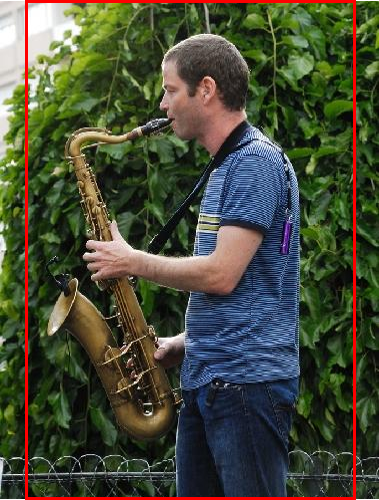
\includegraphics[height=.13\linewidth]{figs/misC2_Photographing_instead_PlayingMusic_img0160.png}
&
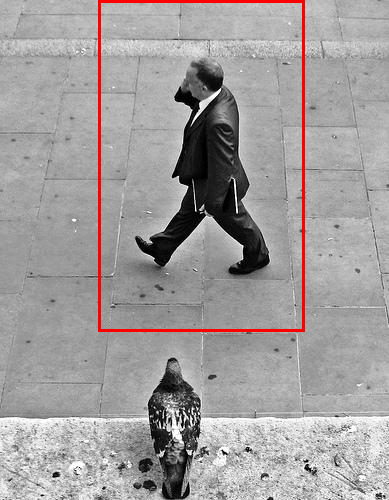
\includegraphics[height=.13\linewidth]{figs/misC2_RidingHorse_instead_Walking_img0073.png}
&
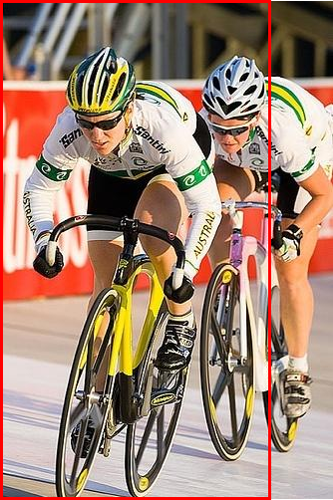
\includegraphics[height=.14\linewidth]{figs/misLSVM_PlayingMusic_instead_RidingBike_img0032.png}
&
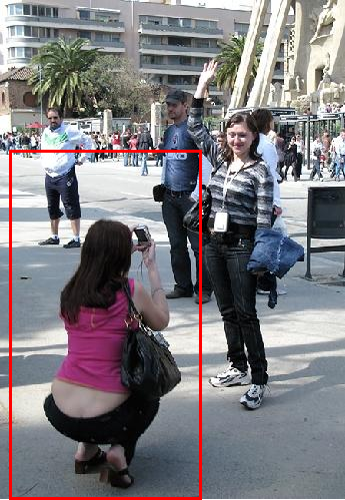
\includegraphics[height=.14\linewidth]{figs/misLSVM_Running_instead_Photographing_img0114.png}
&

\includegraphics[height=.14\linewidth]{figs/misLSVMC2_PlayingMusic_instead_InteractingWithComputer_img0036.png}\\
\hline
\tiny LSVM+C2: & \ok{\tiny PlayingMusic}   & \ok{\tiny Walking}      & \ok{\tiny RidingBike}    & \ok{\tiny Photograph.}  &  \bad{\tiny PlayingMusic} \\ \hline
\tiny C2:      & \bad{\tiny Photograping}  & \bad{\tiny RidingHorse} & \tiny ???                & \tiny ???               & \tiny ???\\ \hline
\tiny LSVM:    & \tiny ???                 & \tiny ???               & \bad{\tiny PlayingMusic} & \bad{\tiny RidingHorse} & \tiny ???\\ \hline
\end{tabular}
\caption{Example of images}
\label{fig:corr1}
\end{figure}
\end{frame}


%==============================================================================
\section{Testing on other databases}
\begin{frame}
\tableofcontents[currentsection]
\end{frame}


\subsection{The sports dataset}
\begin{frame}
\frametitle{The sports dataset}

This is a sports dataset proposed by Gupta \etal with six classes:

\center 
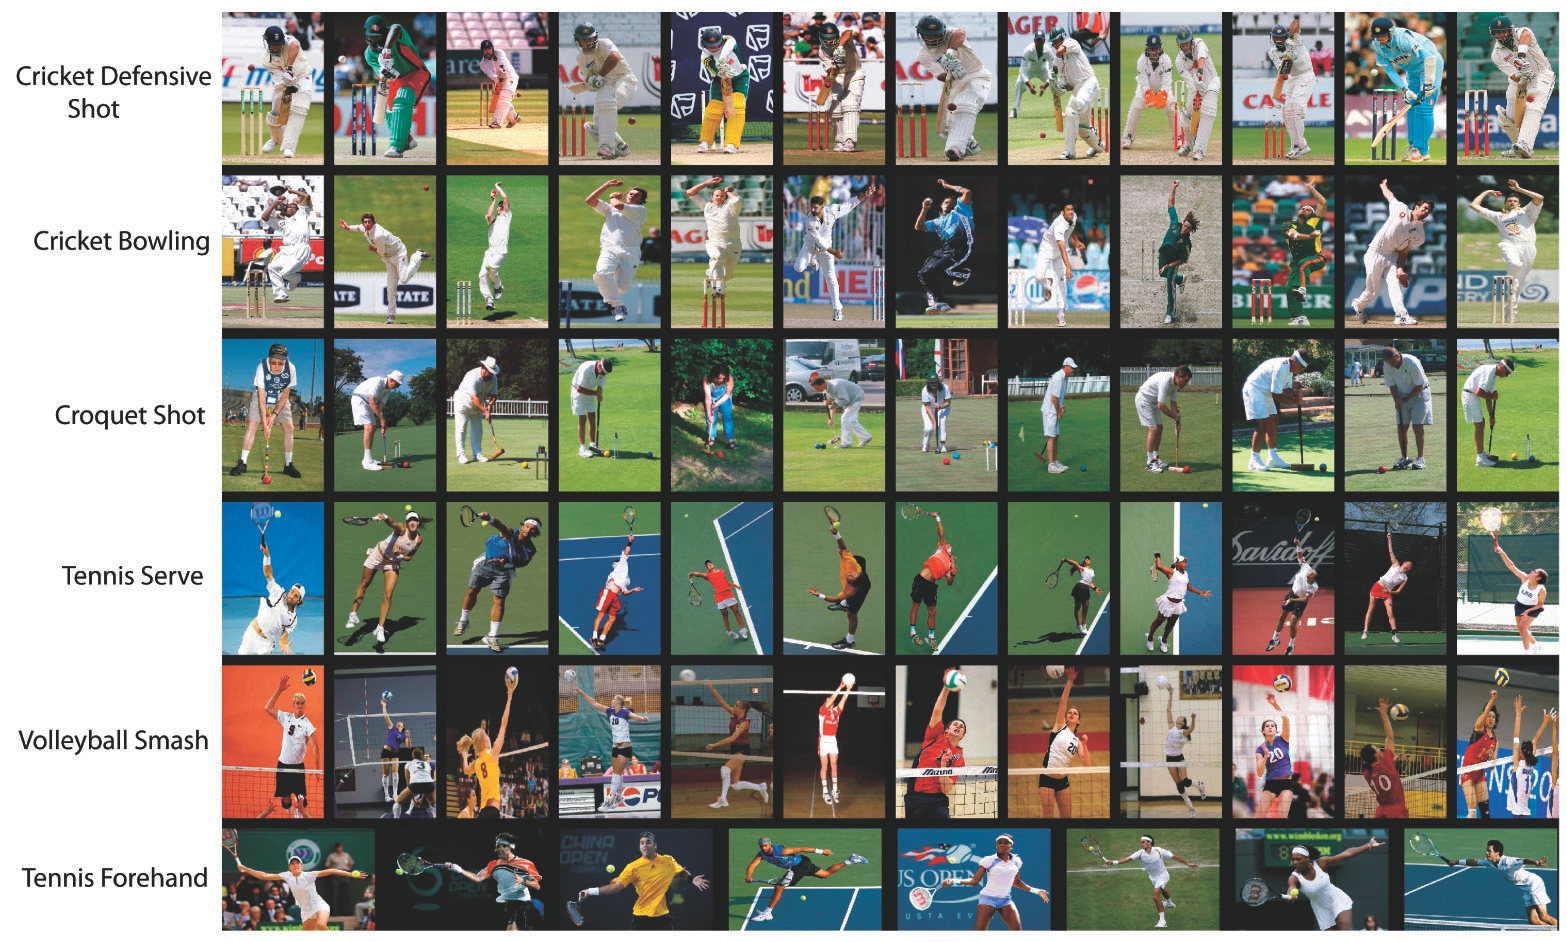
\includegraphics[height=0.6\linewidth]{figs/sport.png}

\end{frame}

%------------------------------------------------------------------------------ 
\begin{frame}
\frametitle{The sports dataset}

We kept the same parameters as the results reported previously:

\begin{table}[t]
\centering
%\rowcolors[]{1}{white}{gray!10}
\begin{tabular}{|l||l|l|}
\hline
Method  				             & mAP	           & Accuracy  \\ \hline 
Gupta~\etal~~\cite{Gupta09}	 & --	             &  $78.67$ \\ \hline 
BOF Image (B) 		 	         &  91.30 	       & ${\bf 85.00} $ \\ \hline 
LSVM 			  		             & 77.19	         & $ 73.33 $ \\ \hline 
LSVM + BOF Image (B)		     & {\bf 91.55}     & $ {\bf 85.00} $ \\ \hline 
\end{tabular}
\caption{Comparison with the method of Gupta~\etal on their dataset.}
\label{tab:gupta}
\end{table}

\end{frame}


%------------------------------------------------------------------------------ 
\subsection{The People-playing-musical-instrument (PPMI) dataset}
\begin{frame}
\frametitle{The People-playing-musical-instrument (PPMI) dataset}

This is a dataset proposed by Fei-Fei \etal with people playing or only holding an instrument.
There are seven different instruments. 

\center 
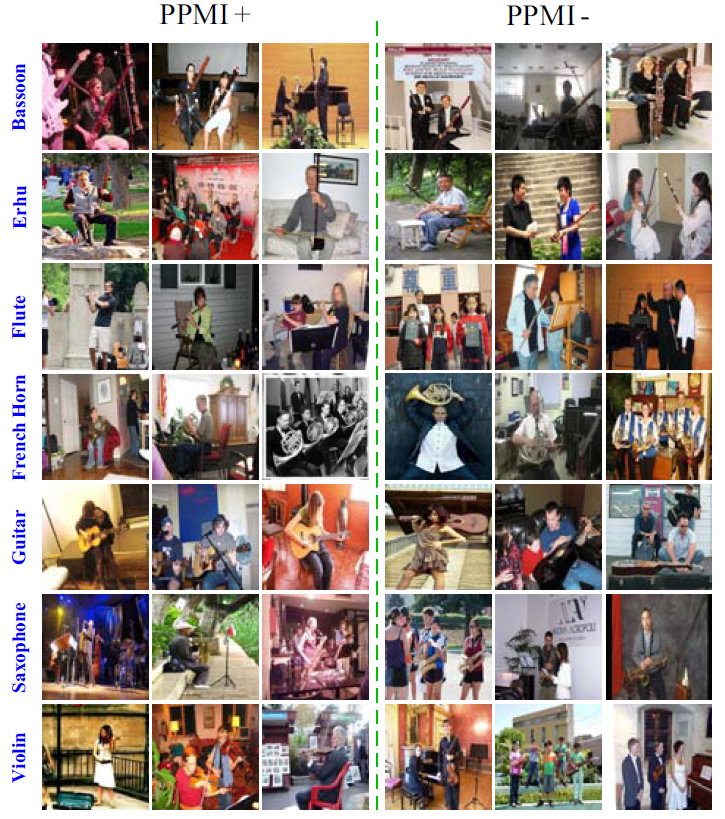
\includegraphics[height=0.6\linewidth]{figs/ppmi.png}

\end{frame}


%------------------------------------------------------------------------------ 
\begin{frame}
\frametitle{The People-playing-musical-instrument (PPMI) dataset}
Results...
\end{frame}

%------------------------------------------------------------------------------ 
\begin{frame}
\frametitle{Conclusion}


\end{frame}

\end{document}
